\chapter{Dialog}
Gesprochene Sprache tritt besonders häufig in Form von \textit{Spontansprache} (z.\,B. im Gegensatz zu Lesesprache) auf, die zudem meistens Teil eines Dialogs ist. Sprachlaute, die in \textit{fließender Rede} in Kombination mit anderen Lauten geäußert werden, weichen in ihrer Form in der Regel von isoliert produzierten Sprachlauten ab (vgl. auch das Kapitel Spontansprachliche Vorgänge), die wiederum der phonetischen Beschreibung zugrunde liegen. Dialoge sind in vielerlei Hinsicht dafür geeignet, spontansprachliche und \textit{suprasegmentale} Eigenschaften in der sprachlichen Kommunikation zu untersuchen, z.\,B. prosodische Mittel zum Halten oder Beenden von \textit{Turns}. Auch in der Sprachtechnologie ($\rightarrow$ Spracherkennung und –synthese) werden zunehmend dialogbasierte Daten berücksichtigt. Viele Kommunikationsmodelle basieren ebenfalls auf dialogisierter Sprache ($\rightarrow$ Psycholinguistik).

\section{Stichworte zur Vorlesung \em{Prosodie und Intonation}}
Grundfrequenz, Tonhöhe, Wortbetonung, Satzakzentuierung, Phrasierung, Deklination, akzent- vs. silbenzählende Sprachen, Paralinguistik... $\rightarrow$ {\tt L7\underline{\ }Prosodie{\&}Intonation.pdf}

\begin{figure}[htbp]
\begin{center}
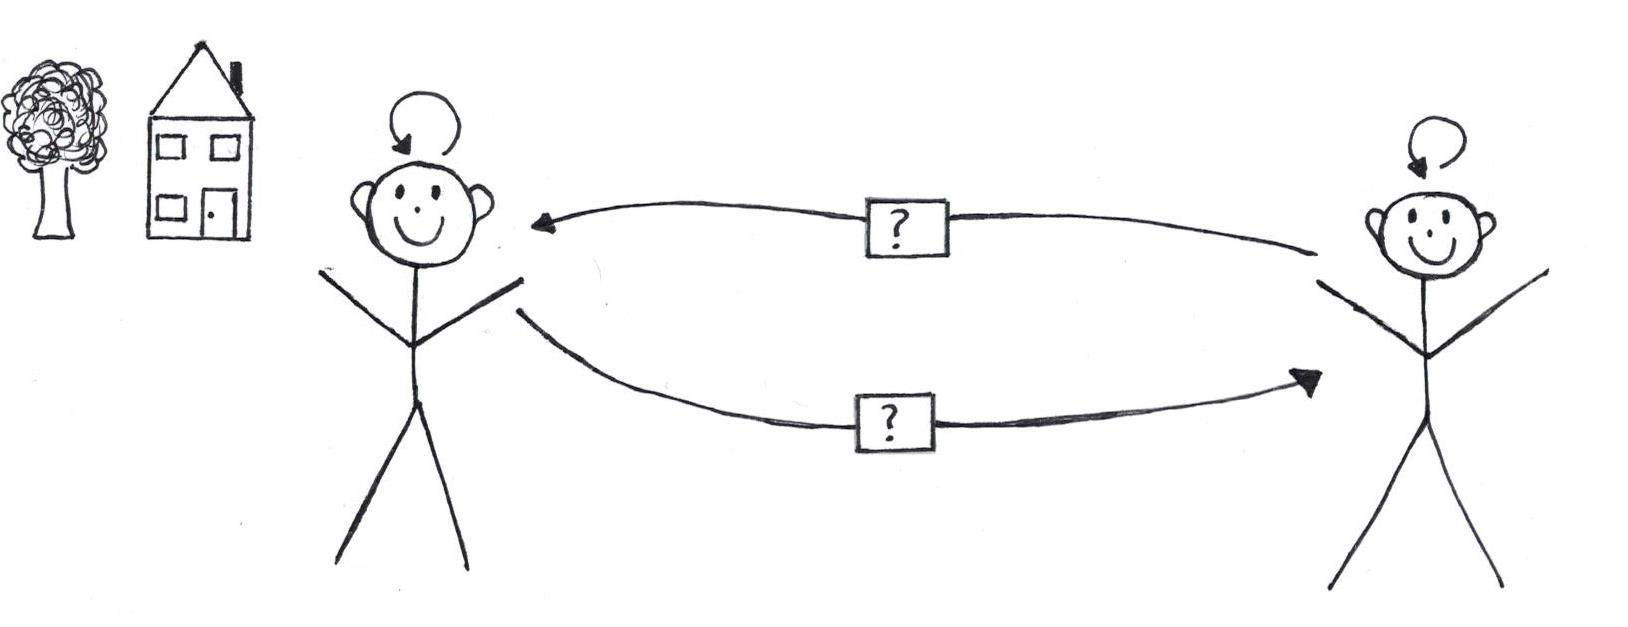
\includegraphics[width=0.6\textwidth]{grafiken/dialog/dialog.jpg}
\label{t5}
\end{center}
\end{figure}


\newpage
\section{Übungen}
1.	Was ist ein Turn? Recherchieren und notieren Sie eine Definition.
\vspace*{3cm}\\

2.	Suchen Sie in Ihren Aufnahmen nach Beispielen für Phrasierungen, die mit der Grammatik (syntaktische Phrase, Komma etc.) (a)  übereinstimmen und (b) von ihr abweichen.
\vspace*{3cm}\\
3.	Prüfen Sie in ihren Aufnahmen, ob Fragen mit einer steigenden oder anderen Grundfrequenz produziert werden.  Notieren Sie Beispiele und beschreiben sie den f0-Verlauf.
\vspace*{3cm}\\

4.	Bei welchen anderen Bereichen der Linguistik sehen Sie Schnittstellen mit der Prosodie und Intonation? Begründen Sie die Vorschläge.\vspace*{1cm}\\
